\graphicspath{{\currfiledir/images/}}

%----------------------------------------------------------------------------------------
%	Caminhos mínimos
%----------------------------------------------------------------------------------------
\chapter{Caminhos mínimos}
Usando-se das propriedades de grafos até agora citados, caminhos mínimos também é uma propriedade que visa, dado dois vértices $v_1$ e $v_2$, buscar qual o caminho mais curto de $v_1$ para $v_2$. O \emph{peso} (\emph{ponderação}) de arestas é outra propriedade adicional para este capítulo. As arestas de um grafo, além de todas as definições previamente definidas, podem ou não possuir peso. Um exemplo da vida real, dado um mapa, os pesos das arestas para um grafo que o representasse poderiam se referir a distância em quilômetros Com isto, o grafo seria classificado como direcionado e ponderado. Quando não se é destacado que o grafo possui pesos, podemos considerar que todas as suas arestas possuem peso 1.

%----------------------------------------------------------------------------------------
%	Algoritmo de Dijkstra
%----------------------------------------------------------------------------------------
\section{Algoritmo de Dijkstra}
O algoritmo de Dijkstra resolve o problema de caminhos mínimos. O algoritmo retorna uma árvore de caminhos mínimos em que um par de nós, raiz da árvore com seus nós filhos, refere-se a um caminho mínimo da raiz ao nó filho em questão.

Do algoritmo, aplicado em grafos:

1) Cria-se um conjunto de árvores de caminhos mínimos (shortest path tree set - sptSet) que mantém o controle dos vértices incluídos na árvore de caminhos mínimos, ou seja, cuja distância mínima da fonte é calculada e finalizada. Inicialmente, este conjunto está vazio.

2) Atribui-se um valor de distância a todos os vértices no grafo de entrada. Inicialmente, todos os valores de distância são definidos como ``INFINITO''. Atribui-se o valor de distância 0 para o vértice de origem para que ele seja selecionado primeiro.

3) Enquanto o sptSet não possui todos os vértices:

    \quad a) É selecionado um vértice $u$ que não está em sptSet e tem um valor de distância mínimo.

    \quad b) Adiciona-se $u$ em sptSet.

    \quad c) Atualiza-se o valor da distância de todos os vértices adjacentes a $u$. Para isto, itera-se em todos os vértices adjacentes e para cada vértice adjacente $v$, se a soma do valor da distância de $u$ (da fonte) e o peso da aresta $(u, v)$, for menor que o valor da distância de $v$, então atualize o valor da distância de $v$.

%----------------------------------------------------------------------------------------
%	Árvore de caminhos mínimos
%----------------------------------------------------------------------------------------
\section{Árvore de caminhos mínimos}
Seguindo-se da definição de árvores de caminhos mínimos proposta em \cite{alane2021}. Uma árvore de caminhos mínimos de um vértice $u$ é uma árvore geradora $T_u$ de $G$, de modo que o caminho de $u$ para todos os outros vértices de $T_u$ é um caminho mínimo em $G$. Tomando-se a árvore de caminho mínimos para um vértice $u$ como sendo $T_u$. Um caminho mínimo que começa na raiz de uma árvore Dijsktra é chamado de ramo de $G$. Mais formalmente, dado $T_u$, para cada $v \neq u$, o caminho mínimo de $u$ a $v$ é um ramo, denotado por $\mathcal{B}_u(v)$. Além disso, cada subcaminho de $\mathcal{B}_u(v) = p_{uv}$ é também um caminho mínimo em $G$, e denotamos esse conjunto de subcaminhos (incluindo $p_{uv}$) como $S(p_{uv})$ ou $S(\mathcal{B}_u(v))$ (ambas as notações são usadas indistintamente, por conveniência). Uma vez que $G$ não é direcionado, o mesmo se aplica a caminhos em ordem reversa, ou seja, cada subcaminho de $p_{vu}$ em $T_u$ também é um caminho mínimo. Com isto, assumimos $S(p_{vu})$ como sendo este conjunto de caminhos mínimos \cite{alane2021}.

%----------------------------------------------------------------------------------------
%	Caminhos mínimos entre todos os pares de vértices (APSP)
%----------------------------------------------------------------------------------------
\section{Caminhos mínimos entre todos os pares de vértices (APSP)}
O APSP, do inglês, {\it all-pairs shortest paths}. é o problema de calcular o comprimento mínimo entre cada par de vértices em um grafo ponderado. O problema APSP é bastante estudado, tendo resultados recentes para uma variedade de suposições para o grafo de entrada (direcionado, não direcionado, ponderado, não ponderado, etc.) \cite{alane2021} \cite{williams2014} \cite{pettie2002}.

\begin{definition}
    (Conjunto de caminhos mínimos de um grafo) O conjunto de $n$ árvores Dijkstra de $G$ é denotado por $\mathcal{T}$. Seja $S(T_u) = \bigcup_{v \in V \backslash\{u\}} (S(p_{uv}) \cup S(P_{vu}))$. O conjunto de caminhos mínimos de um grafo $G$ é definido por $S(G) = \bigcup_{u \in V} S(T_u)$.
\end{definition}

%----------------------------------------------------------------------------------------
%	O algoritmo de Dijkstra para o problema APSP
%----------------------------------------------------------------------------------------
\section{O algoritmo de Dijkstra para o problema APSP}
É possível resolver o problema de encontrar os caminhos mínimos de todos os pares de vértices de um grafo, executando um algoritmo de caminhos mínimos de fonte única $|V|$ vezes, uma vez para cada vértice como fonte. Se todos os pesos das arestas forem não negativos, podemos usar o algoritmo de Dijkstra. Existem variações deste algoritmo, otimizando a complexidade de tempo, sendo o mais famoso deles, o algoritmo de Floyd-Warshall, cuja complexidade de tempo é $\theta(n^3)$ e depende apenas de $n$.

%----------------------------------------------------------------------------------------
%	Centralidade de intermediação (betweenness centrality)
%----------------------------------------------------------------------------------------
\section{Centralidade de intermediação (\emph{betweenness centrality})}
A centralidade de intermediação é uma maneira de detectar a quantidade de influência que um nó tem sobre o fluxo de informações em um grafo. Em outras palavras, usa-se para localizar os nós que servem como ``ponte'' de uma parte de um grafo para outra ou que inferem possuir maior ``importância''.

Com o cálculo de todos os pares de caminhos mínimos em um grafo, os vértices recebem uma pontuação, que se refere a um montante de ``importância'' do nó em relação ao número de caminhos mínimos que passam pelo nó. Em suma, os nós que mais frequentemente estiverem presentes nos caminhos mínimos de um grafo terão pontuações de centralidade de intermediação mais altas.

A Figura~\ref{sec3:graph-betweenness} apresenta um grafo não direcionado colorido com base na centralidade da intermediação de cada vértice do menor (vermelho) ao maior (azul).

\begin{figure}[!htb]
    \centering
    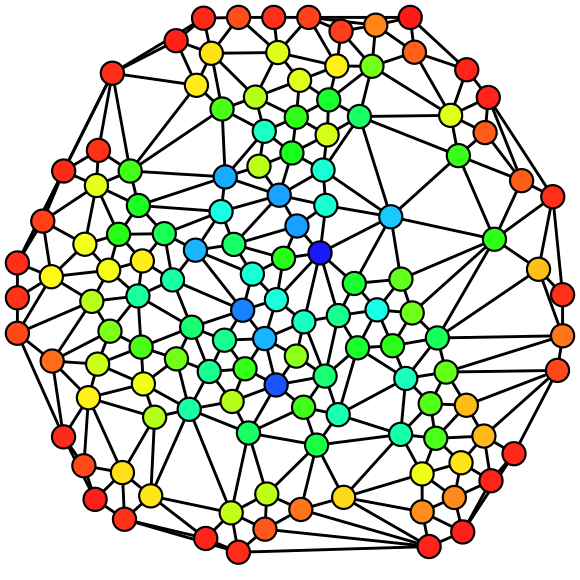
\includegraphics[scale=0.4]{graph-betweenness.png}
    \caption{Grafo não direcionado com as centralidades de intermediação dos vértices.}
    \label{sec3:graph-betweenness}
\end{figure}

Nesta mesma linha, podemos avaliar a ``importância'' de arestas ou, de forma mais relevante, dos caminhos mínimos, atribuindo-lhes pontuações toda vez que estes estão presentes como subcaminhos mínimos em outros caminhos mínimos. Isto desperta a importância e motiva ao estudo de, assim como na centralidade de intermediação em vértices, a centralidade de caminhos mínimos que será discutido na próxima seção.

%----------------------------------------------------------------------------------------
%	Centralidade de caminhos mínimos
%----------------------------------------------------------------------------------------
\section{Centralidade de caminhos mínimos}
A seguir, a definição de centralidade de caminhos mínimos de um grafo, definida em \cite{alane2021}.

\begin{definition}
    (Centralidade de caminhos mínimos) Dado um grafo não direcionado ponderado $G = (V, E)$ com $n = |V|$, um par $(u, v) \in V^2$ e a árvore Dijkstra $T_a$ para cada $a \in V$, sejam $p_{ab} = (a,...,b)$ e $p_{uv} = (u,...,v)$ os caminhos mínimos de $a$ para $b$ e $u$ para $v$, respectivamente, tais que $p_{ab}, p_{uv} \in S(G)$. A centralidade do caminho mínimo de um par $(u, v) \in V^2$ é definida como
    \begin{align*}
        c(u, v) &= \frac{t_{uv}}{n(n - 1)}
    \end{align*}
    onde
    \begin{align*}
        t_{uv} &= \sum_{(a,b) \in V^2 : a \neq b} \mathbb{1}_{\tau_{uv}(\mathcal{B}_a(b))}
    \end{align*}
\end{definition}

A função $\mathbb{1}_{\tau_{uv}(\mathcal{B}_a(b))}$ retorna 1 se houver algum caminho mínimo de $u$ a $v$ como subcaminho do ramo $\mathcal{B}_a(b) \in S (T_a)$ (e 0 caso contrário). Intuitivamente falando, um par $(u, v)$ tem alta centralidade de caminho mínimo se o caminho mínimo $p_{uv} \in S(T_u)$ (e $S(T_v)$) é um subcaminho de um grande número de caminhos mínimos em $S(G)$.

Considere o grafo da Figura~\ref{sec3:grafo-simples-5-nos}. O percurso mais curto do vértice $v_1$ para o vértice $v_3$ é o caminho mínimo $(v_1, v_3)$. Calculando-se todos os possíveis pares de caminhos mínimos deste grafo, chegaremos a conclusão de que o caminho mínimo $(v_1, v_3)$ terá maior centralidade que o caminho mínimo $(v_1, v_5, v_4)$ (percurso mais curto do vértice $v_1$ para o $v_4$) por exemplo, isto porque as vezes em que o caminho mínimo $(v_1, v_3)$ está presente como subcaminho mínimo é maior que as vezes em que o caminho mínimo $(v_1, v_5, v_4)$ está presente em outros.

\begin{figure}[!htb]
    \centering
	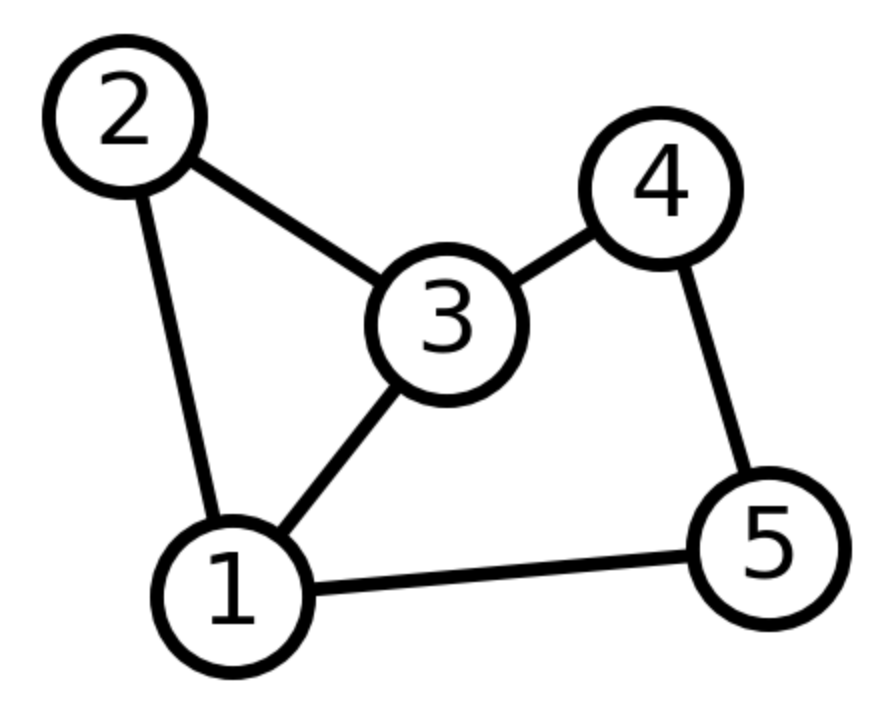
\includegraphics[scale=0.4]{grafo-simples-5-nos.png}
    \caption{Grafo simples com 5 nós.}
    \label{sec3:grafo-simples-5-nos}
\end{figure}

Assim como ocorre com o problema da centralidade de intermediação, a melhor maneira conhecida de se computar a centralidade de caminhos mínimos também é utilizando algoritmos que resolvem o APSP.

%----------------------------------------------------------------------------------------
%	Redundância de caminhos mínimos
%----------------------------------------------------------------------------------------
\section{Redundância de caminhos mínimos}
Adicionalmente, ainda considerando o grafo da Figura~\ref{sec3:grafo-simples-5-nos}, observa-se que do vértice $v_1$ ao vértice $v_4$, um algoritmo de busca por caminhos mínimos pode retornar o percurso mais curto como sendo $(v_1, v_3, v_4)$ ou $(v_1, v_5, v_4)$, porém nos importa apenas uma destas saídas e usaremos a que o algoritmo em questão encontrar. Para a busca de caminhos mínimos, usaremos o algoritmo de Dijkstra e assumiremos seu retorno como verdade. Esta informação é importante e curiosa, pois dependendo de como o algoritmo se comporta/ trata os dados, o resultado do conjunto de caminhos mínimos podem diferir e, consequentemente, os valores de centralidade dos caminhos mínimos nos grafos que possuam mais de uma opção de percurso mais curto entre um par de vértices. Ainda, a aleatorização dos rótulos de um grafo é uma linha de pesquisa neste mesmo escopo que, segundo \cite{alane2021}, em grafos muito esparsos, a aleatorização dos rótulos não resulta em diferenças significativas nos valores de centralidade dos caminhos mínimos.